\section{Traceability Matrices and Graphs}
\label{sec_trace}

The purpose of the traceability matrices is to provide easy references on what
has to be additionally modified if a certain component is changed.  Every time a
component is changed, the items in the column of that component that are marked
with an ``X'' may have to be modified as well.
\begin{itemize}
    \item Table~\ref{tab:traceA} shows the dependencies of Theoretical Models,
    Instance Models, and Likely Changes on the Assumptions
    (\aref{A_TotalFunctions}, \aref{A_formal}, \aref{A_Cognition}, and
    \aref{A_Modular} are excluded from the matrix because they are generally
    applicable)

    \item Table~\ref{tab:traceC} shows the dependencies between Conceptual
    Models

    \item Table~\ref{tab:traceC2Other} shows the dependencies between
    Conceptual Models, Theoretical Models, and Data Types

    \item Table~\ref{tab:traceTY} shows the dependencies between Data Types

    \item Table~\ref{tab:traceIM2T} shows the dependencies of Instance Models
    on Theoretical Models

    \item Table~\ref{tab:traceIM2TY} shows the dependencies of Instance Models
    on Data Types

    \item Table~\ref{tab:traceIM} shows the dependencies between Instance Models

    \item Table~\ref{tab:traceCTY2Reqs} shows the dependencies of Functional
    Requirements on Conceptual Models and Type Definitions

    \item Table~\ref{tab:traceIM2Reqs} shows the dependencies of Functional
    Requirements on Data Constraints and Instance Models

\end{itemize}

\begin{landscape}
    \vspace*{\fill}
    \begin{table}[tbh]
        \centering
        \resizebox{\linewidth}{!}{%
        \begin{tabular}{|c|c|c|c|c|c|c|c|c|c|c|c|c|c|c|c|c|c|c|c|c|c|c|c|}
        \hline

            & \aref{A_Subgoal} & \aref{A_Goal2Emotion} & \aref{A_OneState}
            & \aref{A_EmotionTypeIntensity} & \aref{A_AppraisalProcess} &
            \aref{A_Goal2Intensity} & \aref{A_Surprise} &
            \aref{A_Surprise2} & \aref{A_Interest} & \aref{A_Acceptance} &
            \aref{A_DecaySpeed} & \aref{A_Equilibrium} & \aref{A_DecayRate}
            & \aref{A_DecayUnique} & \aref{A_OnePADPoint} &
            \aref{A_EmotionTerms} & \aref{A_PADStats} &
            \aref{A_LimitIntensity} & \aref{A_PositiveIntensity} &
            \aref{A_EmotionPairs} & \aref{A_Events} &
            \aref{A_GustatoryGoal} & \aref{A_UpdateEmotionState} \\\hline

            \tref{T_CalculateEmotionGP} & X & X & X & X & X &  &  &  &  &
            &  &  &  &  &  &  &  &  &  &  &  & &  \\\hline

            \tref{T_CalculateEmotionIntensity} &  &  &  &  &  & X &  &  &
            &  &  &  &  &  &  &  &  &  &  &  &  & &  \\\hline

            \tref{T_CalculateEmotionSurprise} &  &  &  &  &  &  & X & X &
            &  &  &  &  &  &  &  &  &  &  &  &  & &  \\\hline

            \tref{T_CalculateEmotionInterest} &  &  &  &  &  &  &  &  & X
            &  &  &  &  &  &  &  &  &  &  &  &  & &  \\\hline

            \tref{T_CalculateEmotionAcceptance} &  &  &  &  &  &  &  &  &
            & X &  &  &  &  &  &  &  &  &  &  &  & &  \\\hline

            \tref{T_DecayEmotionState} &  &  &  &  &  &  &  &  &  &  & X &
            X & X & X &  &  &  &  &  &  &  & &  \\\hline

            \tref{T_GetEmotionStatePAD} &  &  &  &  &  &  &  &  &  &  &  &
            &  &  & X & X & X &  &  &  &  & &  \\\hline

            \tyref{TY_EmotionIntensity} &  &  &  &  &  &  &  &  &  &  &  &
            &  &  &  &  &  &  & X &  &  & &  \\\hline

            \tyref{TY_EmotionState} &  &  &  &  &  &  &  &  &  &  &  &
            &  &  &  &  &  & X &  & X &  & &  \\\hline

            \tyref{TY_EmotionDecayState} &  &  &  &  &  &  &  &  &  &  &
            &  &  &  &  &  &  &  & X &  &  & &  \\\hline

            \tyref{TY_Goal} &  &  &  &  &  &  &  &  &  &  &  &  &  &  &  &
            &  &  &  &  & X & &  \\\hline

            \iref{IM_CalculateEmotionGP} &  &  &  &  &  &  &  &  &  &  &
            &  &  &  &  &  &  &  &  &  &  & X &  \\\hline

            \iref{IM_UpdateEmotionState} &  &  &  &  &  &  &  &  &  &  &
            &  &  &  &  &  &  &  &  &  &  & & X \\\hline

            \lcref{LC_Subgoal} & X &  &  &  &  &  &  &  &  &  &  &  &  &
            &  &  &  &  &  &  &  & &  \\\hline

            \lcref{LC_Goal2Emotion} &  & X &  &  &  &  &  &  &  &  &  &  &
            &  &  &  &  &  &  &  &  & &  \\\hline

            \lcref{LC_EmotionTypeIntensity} &  &  &  & X &  &  &  &  &  &
            &  &  &  &  &  &  &  &  &  &  &  & &  \\\hline

            \lcref{LC_Goal2Intensity} &  &  &  &  &  & X &  &  &  &  &  &
            &  &  &  &  &  &  &  &  &  & &  \\\hline

            \lcref{LC_Surprise} &  &  &  &  &  &  & X & X &  &  &  &  &  &
            &  &  &  &  &  &  &  & &  \\\hline

            \lcref{LC_Interest} &  &  &  &  &  &  &  &  & X &  &  &  &  &
            &  &  &  &  &  &  &  & &  \\\hline

            \lcref{LC_DecaySpeed} &  &  &  &  &  &  &  &  &  &  & X &  &
            &  &  &  &  &  &  &  &  & &  \\\hline

            \lcref{LC_Equilibrium} &  &  &  &  &  &  &  &  &  &  &  & X &
            &  &  &  &  &  &  &  &  & &  \\\hline

            \lcref{LC_DecayRate} &  &  &  &  &  &  &  &  &  &  &  &  & X &
            &  &  &  &  &  &  &  & &  \\\hline

            \lcref{LC_EmotionTerms} &  &  &  &  &  &  &  &  &  &  &  &  &
            &  &  & X &  &  &  &  &  & &  \\\hline

            \lcref{LC_PADStats} &  &  &  &  &  &  &  &  &  &  &  &  &  &
            &  &  & X &  &  &  &  & &  \\\hline

            \lcref{LC_PositiveIntensity} &  &  &  &  &  &  &  &  &  &  &
            &  &  &  &  &  &  &  & X &  &  & &  \\\hline

            \lcref{LC_EmotionPairs} &  &  &  &  &  &  &  &  &  &  &  &  &
            &  &  &  &  &  &  & X &  & &  \\\hline

            \lcref{LC_UpdateEmotionState} &  &  &  &  &  &  &  &  &  &  &
            &  &  &  &  &  &  &  &  &  &  & & X \\\hline

        \end{tabular}%
        }
        \caption{Traceability between Assumptions and Other Items}
        \label{tab:traceA}
    \end{table}
    \vspace*{\fill}
\end{landscape}

\vspace*{\fill}
\begin{table}[tbh]
    \centering
    \begin{tabular}{|c|c|c|c|c|c|c|c|c|c|c|c|c|c|}
        \hline

        & \cref{C_Emotion} & \cref{C_EmotionStruct} &
        \cref{C_ComplexEmotion} & \cref{C_ComplexEmotions-CTE} &
        \cref{C_PAD} & \cref{C_Appraisal-CTE} & \cref{C_EmOther} &
        \cref{C_EmIntensity-CTE} & \cref{C_EmDecay} & \cref{C_Goals} &
        \cref{C_Plans} & \cref{C_Attention} & \cref{C_Relation-CTE} \\
        \hline

        \cref{C_Emotion} & X &  &  &  &  &  &  &  &  & X &  &  &  \\ \hline

        \cref{C_EmotionStruct} &  & X &  &  &  &  &  &  &  &  &  &  &  \\
        \hline

        \cref{C_ComplexEmotion} &  & X & X &  &  &  &  &  &  &  &  &  &  \\
        \hline

        \cref{C_ComplexEmotions-CTE} &  &  &  & X &  & X &  &  &  &  &  &
        & X \\ \hline

        \cref{C_PAD} &  &  &  &  & X &  &  &  &  &  &  &  &  \\ \hline

        \cref{C_Appraisal-CTE} &  &  &  &  &  & X &  &  &  & X & X &  &  \\
        \hline

        \cref{C_EmOther} &  &  &  &  &  & X & X &  &  &  &  & X &  \\ \hline

        \cref{C_EmIntensity-CTE} & X &  &  &  &  & X &  & X &  &  &  &  &
        \\ \hline

        \cref{C_EmDecay} & X &  &  &  &  &  &  &  & X &  &  &  &  \\ \hline

        \cref{C_Goals} &  &  &  &  &  &  &  &  &  & X &  &  &  \\ \hline

        \cref{C_Plans} &  &  &  &  &  &  &  &  &  & X & X &  &  \\ \hline

        \cref{C_Attention} &  &  &  &  &  &  &  &  &  &  &  & X &  \\ \hline

        \cref{C_Relation-CTE} &  &  &  &  &  &  &  &  &  &  &  &  & X \\
        \hline
    \end{tabular}
    \caption{Traceability between Conceptual Models}
    \label{tab:traceC}
\end{table}
\vspace*{\fill}

\begin{landscape}
    \vspace*{\fill}
    \begin{table}[tbh]
        \centering
        \begin{tabular}{|c|c|c|c|c|c|c|c|c|c|c|c|c|c|c|c|c|c|c|c|c|}
            \hline

            & \cref{C_Emotion} & \cref{C_EmotionStruct} &
            \cref{C_ComplexEmotion} & \cref{C_ComplexEmotions-CTE} &
            \cref{C_PAD} & \cref{C_Appraisal-CTE} & \cref{C_EmOther} &
            \cref{C_EmIntensity-CTE} & \cref{C_EmDecay} & \cref{C_Goals} &
            \cref{C_Plans} & \cref{C_Attention} & \cref{C_Relation-CTE} &
            \tref{T_CalculateEmotionGP} & \tref{T_CalculateEmotionIntensity} &
            \tref{T_CalculateEmotionSurprise} &
            \tref{T_CalculateEmotionInterest} &
            \tref{T_CalculateEmotionAcceptance} & \tref{T_DecayEmotionState} &
            \tref{T_GetEmotionStatePAD} \\ \hline

            \tref{T_CalculateEmotionGP} &  &  &  &  &  & X &  &  &  & X & X &
            &  & X &  &  &  &  &  & \\ \hline

            \tref{T_CalculateEmotionIntensity} &  &  &  &  &  &  &  & X &  &
            &  &  & &  & X &  &  &  &  &  \\ \hline

            \tref{T_CalculateEmotionSurprise} &  &  &  &  &  &  & X &  &  &  &
            &  & &  &  & X &  &  &  &  \\ \hline

            \tref{T_CalculateEmotionInterest} &  &  &  &  &  &  & X &  &  &  &
            &  & &  &  &  & X &  &  &  \\ \hline

            \tref{T_CalculateEmotionAcceptance} &  &  &  & X &  &  &  &  &  &
            &  &  & X &  &  &  &  & X &  & \\ \hline

            \tref{T_DecayEmotionState} &  &  &  &  &  &  &  &  & X &  &  &  &
            &  &  &  &  &  & X &  \\ \hline

            \tref{T_GetEmotionStatePAD} &  & X &  &  & X &  &  &  &  &  &  &  &
             &  &  &  &  &  &  &  \\ \hline

            \tyref{TY_EmotionIntensity} &  &  &  &  &  &  &  &  &  &  &  &  &
            &  & X & X & X & X &  &  \\ \hline

            \tyref{TY_EmotionDecay} &  &  &  &  &  &  &  &  &  &  &  &  &  &
            &  &  &  &  & X &  \\ \hline

            \tyref{TY_EmotionKind} &  & X &  &  &  &  &  &  &  &  &  &  &  &
            &  &  &  &  &  &  \\ \hline

            \tyref{TY_EmotionState} & X &  &  &  &  &  &  &  &  &  &  &  & &
            &  &  &  &  &  &  \\\hline

            \tyref{TY_EmotionDecayState} &  &  &  &  &  &  &  &  &  &  &  &  &
            &  &  &  &  &  & X &  \\\hline

            \tyref{TY_Emotion} & X &  &  &  &  &  &  &  &  &  &  &  & &  &  &
            &  &  &  &  \\ \hline

            \tyref{TY_PAD} &  &  &  &  & X &  &  &  &  &  &  &  & &  &  &
            &  &  &  &  \\ \hline

            \tyref{TY_WorldState} &  &  &  &  &  &  &  &  &  &  &  &  & &  &
            &  & &  &  &  \\ \hline

            \tyref{TY_WorldStateChange} &  &  &  &  &  &  &  &  &  &  &  &  &
            &  &  &  &  &  &  &  \\ \hline

            \tyref{TY_DistanceBetweenWorldStates} &  &  &  &  &  &  &  &  &  &
            &  &  & &  &  &  &  &  &  &  \\ \hline

            \tyref{TY_DistanceBetweenWorldStatesChange} &  &  &  &  &  &  &  &
            &  & X &  &  & &  &  &  &  &  &  &  \\ \hline

            \tyref{TY_Goal} &  &  &  &  &  &  &  &  &  & X &  &  & &  &  &  &
            &  &  &  \\ \hline

            \tyref{TY_Plan} &  &  &  &  &  &  &  &  &  &  & X &  & &  &  &  &
            &  &  &  \\ \hline

            \tyref{TY_Attention} &  &  &  &  &  &  &  &  &  &  &  & X & &  &
            &  &  &  &  &  \\ \hline

            \tyref{TY_Relation-CTE} &  &  &  &  &  &  &  &  &  &  &  &  & X &
            &  &  &  &  &  &  \\ \hline

        \end{tabular}
        \caption{Traceability between Conceptual Models, Theoretical Models,
        and Data Types}
        \label{tab:traceC2Other}
    \end{table}
    \vspace*{\fill}
\end{landscape}

\begin{landscape}
    \vspace*{\fill}
    \begin{table}[tbh]
        \centering
        \resizebox{\linewidth}{!}{%
        \begin{tabular}{|c|c|c|c|c|c|c|c|c|c|c|c|c|c|c|c|c|c|}
            \hline

            & \tyref{TY_Time} & \tyref{TY_EmotionIntensity} &
            \tyref{TY_DeltaIntensity} & \tyref{TY_EmotionDecay} &
            \tyref{TY_EmotionKind} & \tyref{TY_EmotionState} &
            \tyref{TY_EmotionDecayState} & \tyref{TY_Emotion} & \tyref{TY_PAD}
            & \tyref{TY_WorldState} & \tyref{TY_WorldStateChange} &
            \tyref{TY_DistanceBetweenWorldStates} &
            \tyref{TY_DistanceBetweenWorldStatesChange} & \tyref{TY_Goal} &
            \tyref{TY_Plan} & \tyref{TY_Attention} & \tyref{TY_Relation-CTE}
            \\\hline

            \tyref{TY_Time} & X &  &  &  &  & && &  & & & & & & & & \\\hline

            \tyref{TY_EmotionIntensity} && X &&  &  &  &&  &  &  && & & & & &
            \\\hline

            \tyref{TY_DeltaIntensity} && X & X & &  &  &  & &  &  &  & & & & &
            & \\\hline

            \tyref{TY_EmotionDecay} & &&& X &  &  &  &  &&  &  & & & & & &
            \\\hline

            \tyref{TY_EmotionKind}  && & & & X &  &  &  &&  & & & & & & &
            \\\hline

            \tyref{TY_EmotionState} && X &  &  & X & X &  & &  &  &  & & & & & &
            \\\hline

            \tyref{TY_EmotionDecayState} && X &  & X & X &  & X & &  &  &  & & &
            & & & \\\hline

            \tyref{TY_Emotion} & X &  &&&  & X &  & X & &  &  & & & & & &
            \\\hline

            \tyref{TY_PAD} &  &  &&&  &  &  &  & X &  &  & & & & & &\\\hline

            \tyref{TY_WorldState} &  &  &  &  &  & && &  & X & & & && & &
            \\\hline

            \tyref{TY_WorldStateChange} &  &  &  &  &  & && &  &  & X & & && &
            & \\\hline

            \tyref{TY_DistanceBetweenWorldStates} &  &  &  &  &  & && &  & X &
            & X & && & & \\\hline

            \tyref{TY_DistanceBetweenWorldStatesChange} &  &  &  &  &  & && &
            & X & X &  & X & & && \\\hline

            \tyref{TY_Goal} &&  &  &  & && & &  & X & X & X & X & X &
            &&\\\hline

            \tyref{TY_Plan} &  &  &&&  &  &  & &  & X & X &  &  & X & X & &
            \\\hline

            \tyref{TY_Attention} & X & &  &  &  &  & & & & &  &&& & & X
            & \\\hline

            \tyref{TY_Relation-CTE} &  &  &  &  &  &&&& & & & &  & &&& X
            \\\hline

        \end{tabular}%
        }
        \caption{Traceability between Data Types}
        \label{tab:traceTY}
    \end{table}
    \vspace*{\fill}
\end{landscape}

\vspace*{\fill}
\begin{table}[tbh]
    \centering
        \begin{tabular}{|c|c|c|c|c|c|c|c|}
            \hline

            & \tref{T_CalculateEmotionGP} &
            \tref{T_CalculateEmotionIntensity} &
            \tref{T_CalculateEmotionSurprise} &
            \tref{T_CalculateEmotionInterest} &
            \tref{T_CalculateEmotionAcceptance} &
            \tref{T_DecayEmotionState} & \tref{T_GetEmotionStatePAD} \\\hline

            \iref{IM_CalculateEmotionGP} & X &  &  &  &  & & \\\hline

            \iref{IM_CalculateEmotionSurpriseElicit} &  &  & X &  & & &
            \\\hline

            \iref{IM_CalculateEmotionInterestElicit} &  &  &  & X &  &  &
            \\\hline

            \iref{IM_CalculateEmotionAcceptanceElicit} &  &  &  &  & X & &
            \\\hline

            \iref{IM_CalculateEmotionIntensity} &  & X &  &  &  &  & \\\hline

            \iref{IM_CalculateEmotionSurprise} &  &  & X &  &  & & \\\hline

            \iref{IM_CalculateEmotionInterest} &  &  &  & X &  & & \\\hline

            \iref{IM_CalculateEmotionAcceptance} &  &  &  &  & X & & \\\hline

            \iref{IM_DecayEmotionState} & &  & &  &  & X & \\\hline

            \iref{IM_UpdateEmotionState} &&  & & &  &  &  \\\hline

            \iref{IM_UpdateEmotionState2} & &&&  &  &  &   \\\hline

            \iref{IM_UpdateEmotion}  && & & &  &  &  \\\hline

            \iref{IM_GetEmotionState} &&  &  &  &  &  &  \\\hline

            \iref{IM_DecayEmotion} &&  &  &  &  &  &   \\\hline

            \iref{IM_GetEmotionStatePAD} &  &  &&&  &  & X \\\hline

        \end{tabular}
    \caption{Traceability between Instance and Theoretical Models}
    \label{tab:traceIM2T}
\end{table}
\vspace*{\fill}

\begin{landscape}
    \vspace*{\fill}
    \begin{table}[tbh]
        \centering
        \begin{tabular}{|c|c|c|c|c|c|c|c|c|c|c|c|c|c|c|c|c|c|}
            \hline

            & \tyref{TY_Time} & \tyref{TY_EmotionIntensity} &
            \tyref{TY_DeltaIntensity} & \tyref{TY_EmotionDecay} &
            \tyref{TY_EmotionKind} & \tyref{TY_EmotionState} &
            \tyref{TY_EmotionDecayState} & \tyref{TY_Emotion} & \tyref{TY_PAD}
            & \tyref{TY_WorldState} & \tyref{TY_WorldStateChange} &
            \tyref{TY_DistanceBetweenWorldStates} &
            \tyref{TY_DistanceBetweenWorldStatesChange} & \tyref{TY_Goal} &
            \tyref{TY_Plan} & \tyref{TY_Attention} & \tyref{TY_Relation-CTE}
            \\\hline

            \iref{IM_CalculateEmotionGP} &  &  &  &  & X & && &  & X & X & X &
            X & X & X & & \\\hline

            \iref{IM_CalculateEmotionSurpriseElicit} & X &  &  &  &  & &&
            &  & &  & & & & & &  \\\hline

            \iref{IM_CalculateEmotionInterestElicit} &  &  &  &  &  & &&
            &  & & & & & & & X & \\\hline

            \iref{IM_CalculateEmotionAcceptanceElicit} &  & X & X &  &  &
            && &  & & & & & & & & X \\\hline

            \iref{IM_CalculateEmotionIntensity} &  &  & X &  &  & && &  & X
            & X & & & X & & &  \\\hline

            \iref{IM_CalculateEmotionSurprise} & X &  & X &  &  & && &  & &
            & & & & & & \\\hline

            \iref{IM_CalculateEmotionInterest} &  &  & X &  &  & && &  & &
            & & & & & X & \\\hline

            \iref{IM_CalculateEmotionAcceptance} &  &  & X &  &  & && &  &
            & & & & & & & X \\\hline

            \iref{IM_DecayEmotionState} & X & X && X &  &  &&  &  &  && & & &
            & &  \\\hline

            \iref{IM_UpdateEmotionState} && X & X & & X &  &  & &  &  &  & &
            && & & \\\hline

            \iref{IM_UpdateEmotionState2} & & X &&  & X & X &  &  &&  &  & & &
            &  & & \\\hline

            \iref{IM_UpdateEmotion} & X & & & &  & X &  & X &&  & & & & &  & &
            \\\hline

            \iref{IM_GetEmotionState} & X &  &  &  & & X &  & X &  &  &  & &
            &  & & & \\\hline

            \iref{IM_DecayEmotion} & X &  &  &  & X & X & X & X &  &  &
            & & & & & & \\\hline

            \iref{IM_GetEmotionStatePAD} &  &  &&& X & X &  &  & X &  &  & &
            & &  & &  \\\hline

        \end{tabular}
        \caption{Traceability between Instance Models and Data Types}
        \label{tab:traceIM2TY}
    \end{table}
    \vspace*{\fill}
\end{landscape}

\begin{landscape}
    \vspace*{\fill}
    \begin{table}[tbh]
        \centering
        \begin{tabular}{|c|c|c|c|c|c|c|c|c|c|c|c|c|c|c|c|}
            \hline

            & \iref{IM_CalculateEmotionGP} &
            \iref{IM_CalculateEmotionSurpriseElicit} &
            \iref{IM_CalculateEmotionInterestElicit} &
            \iref{IM_CalculateEmotionAcceptanceElicit} &
            \iref{IM_CalculateEmotionIntensity} &
            \iref{IM_CalculateEmotionSurprise} &
            \iref{IM_CalculateEmotionInterest} &
            \iref{IM_CalculateEmotionAcceptance} & \iref{IM_DecayEmotionState}
            & \iref{IM_UpdateEmotionState} & \iref{IM_UpdateEmotionState2} &
            \iref{IM_UpdateEmotion} & \iref{IM_GetEmotionState} &
            \iref{IM_DecayEmotion} & \iref{IM_GetEmotionStatePAD} \\\hline

            \iref{IM_CalculateEmotionGP} & X &  &  &  &  & && &  &  &  &  &  &
            & \\\hline

            \iref{IM_CalculateEmotionSurpriseElicit} &  & X &  &  &  & &&
            &  & &  & & & & \\\hline

            \iref{IM_CalculateEmotionInterestElicit} &  &  & X &  &  & &&
            &  & & & & & & \\\hline

            \iref{IM_CalculateEmotionAcceptanceElicit} &  &  &  & X &  &
            && &  & & & & & & \\\hline

            \iref{IM_CalculateEmotionIntensity} &  &  &  &  & X & && &  &
            &  & & &  & \\\hline

            \iref{IM_CalculateEmotionSurprise} &  &  &  &  &  & X && &  & &
            & & & & \\\hline

            \iref{IM_CalculateEmotionInterest} &  &  &  &  &  & & X & &  & &
            & & & & \\\hline

            \iref{IM_CalculateEmotionAcceptance} &  &  &  &  &  & && X &  &
            & & & & & \\\hline

            \iref{IM_DecayEmotionState} &  &  &&  &  &  &&  & X &  && & & &
            \\\hline

            \iref{IM_UpdateEmotionState} &&  &  & &  &  &  & &  & X &  & &
            && \\\hline

            \iref{IM_UpdateEmotionState2} & &  &&  &  &  &  &  &&  & X & & &
            & \\\hline

            \iref{IM_UpdateEmotion} &  & & & &  &  &  &  &&  & & X & & &
            \\\hline

            \iref{IM_GetEmotionState} &  &  &  &  & &  &  &  &  &  &  & & X &
            & \\\hline

            \iref{IM_DecayEmotion} &  &  &  &  &  &  &  &  & X &  & X & & X & X
            & \\\hline

            \iref{IM_GetEmotionStatePAD} &  &  &&&  &  &  &  &  &  &  & & & & X
            \\\hline

        \end{tabular}
        \caption{Traceability between Instance Models}
        \label{tab:traceIM}
    \end{table}
    \vspace*{\fill}
\end{landscape}

\begin{landscape}
    \vspace*{\fill}
\begin{table}[tbh]
    \centering
    \resizebox{\linewidth}{!}{%
    \begin{tabular}{|c|c|c|c|c|c|c|c|c|c|c|c|c|c|c|c|c|c|c|c|}
        \hline

        & \cref{C_ComplexEmotion} & \cref{C_ComplexEmotions-CTE} &
        \tyref{TY_Time} & \tyref{TY_EmotionIntensity} &
        \tyref{TY_DeltaIntensity} & \tyref{TY_EmotionDecay} &
        \tyref{TY_EmotionKind} & \tyref{TY_EmotionState} &
        \tyref{TY_EmotionDecayState} & \tyref{TY_Emotion} & \tyref{TY_PAD} &
        \tyref{TY_WorldState} & \tyref{TY_WorldStateChange} &
        \tyref{TY_DistanceBetweenWorldStates} &
        \tyref{TY_DistanceBetweenWorldStatesChange} & \tyref{TY_Goal} &
        \tyref{TY_Plan} & \tyref{TY_Attention} & \tyref{TY_Relation-CTE}
        \\\hline

        \rref{R_TimeType} &  &  & X &  &  & &  & &  & & & && & & & & & \\\hline

        \rref{R_IntensityTypeUse} &  &  &  & X &  & &  & &  & & & && & & & & &
        \\\hline

        \rref{R_IntensityChangeType} &  &  &  &  & X & &  & &  & & & && & & & &
        & \\\hline

        \rref{R_IntensityDecayType} &  &  &  &  &  & X &  & &  & & & && & & & &
        & \\\hline

        \rref{R_EmotionKindsType} &  &  &  &  &  &  & X & &  & & & && & & & &
        & \\\hline

        \rref{R_EmotionStateType} &  &  &  &  &  &  &  & X &  & & & && & & & &
        & \\\hline

        \rref{R_EmotionDecayStateType} &  &  &  &  &  &  &  &  & X & & & && & &
        & & &  \\\hline

        \rref{R_EmotionType} &  &  &  &  &  &  &  &  &  & X & & && & &  & &  &
        \\\hline

        \rref{R_PADPointType} &  &  &  &  &  &  &  &  &  &  & X & && & &  & &
        & \\\hline

        \rref{R_WorldType} &  &  &  &  &  &  &  &  &  &  &  & X && & & & &  &
        \\\hline

        \rref{R_WorldChangeType} &  &  &  &  &  &  &  &  &  &  &  &  & X & & &
        & &  &  \\\hline

        \rref{R_DistanceType} &  &  &  &  &  &  &  &  &  &  &  &  &  & X & &
        & &  & \\\hline

        \rref{R_DistanceChangeType} &  &  &  &  &  &  &  &  &  &  &  &  &  & &
        X &  & &  & \\\hline

        \rref{R_GoalType} &  &  &  &  &  &  &  &  &  &  &  &  &  & &  & X & &
        & \\\hline

        \rref{R_PlanType} &  &  &  &  &  &  &  &  &  &  &  &  &  & &  &  & X &
        &  \\\hline

        \rref{R_Attention} &  &  &  &  &  &  &  &  &  &  &  &  &  & &  &  &  &
        X &  \\\hline

        \rref{R_SocialAttachment} &  &  &  &  &  & &  & &  & & & && & & & & & X
        \\\hline

        \rref{R_MixingEmotionsPES} & X &  &  & X &  & & X & &  & & & && & & & &
        & \\\hline

        \rref{R_PartitionEmotions} & X &  &  & X &  & & X & &  & & & && & & & &
        &  \\\hline

        \rref{R_MixingEmotionsCTE} &  & X &  &  &  & & X & &  & & & && & & & &
        & \\\hline

    \end{tabular}%
}
    \caption{Traceability between Conceptual Models, Type Definitions, and
    Requirements}
    \label{tab:traceCTY2Reqs}
    \end{table}
\vspace*{\fill}
\end{landscape}

\begin{landscape}
    \vspace*{\fill}
\begin{table}[tbh]
    \centering
    \begin{tabular}{|c|c|c|c|c|c|c|c|c|c|c|c|c|c|c|c|c|}
        \hline

        & \ref{sec_DataConstraints} & \iref{IM_CalculateEmotionGP} &
        \iref{IM_CalculateEmotionSurpriseElicit} &
        \iref{IM_CalculateEmotionInterestElicit} &
        \iref{IM_CalculateEmotionAcceptanceElicit} &
        \iref{IM_CalculateEmotionIntensity} &
        \iref{IM_CalculateEmotionSurprise} &
        \iref{IM_CalculateEmotionInterest} &
        \iref{IM_CalculateEmotionAcceptance} & \iref{IM_DecayEmotionState}
        & \iref{IM_UpdateEmotionState} & \iref{IM_UpdateEmotionState2} &
        \iref{IM_UpdateEmotion} & \iref{IM_GetEmotionState} &
        \iref{IM_DecayEmotion} & \iref{IM_GetEmotionStatePAD} \\\hline

        \rref{R_Types} & X &  &  &  &  &  &  &  &  &  &  &  && & & \\\hline

        \rref{R_GenerateEmotionCTE} &  & X & X & X & X & &  & &  & & & && & &
        \\\hline

        \rref{R_CalculateIntensity} &  &  &  &  &  & X & X & X & X & & & && &
        &  \\\hline

        \rref{R_DecayIntensity} &  &  &  &  &  & &  & &  & X & & && & &
        \\\hline

        \rref{R_DecayEmotion} &  &  &  &  &  & &  & &  & & & && & X &  \\\hline

        \rref{R_UpdateAnIntensity} &  &  &  &  &  & &  & &  & & X & && & &
        \\\hline

        \rref{R_UpdateEmotionState} &  &  &  &  &  & &  & &  & &  & X && & &
        \\\hline

        \rref{R_UpdateEmotion} &  &  &  &  &  & &  & &  & &  &  & X & & &
        \\\hline

        \rref{R_GetEmotionState} &  &  &  &  &  & &  & &  & &  &  &  & X & &
        \\\hline

        \rref{R_Convert2PAD} &  &  &  &  &  & &  & &  & & & && & & X \\\hline

    \end{tabular}
    \caption{Traceability between Data Constraints, Instance Models, and
    Requirements}
    \label{tab:traceIM2Reqs}
\end{table}
\vspace*{\fill}
\end{landscape}

The purpose of the traceability graphs is to provide a difference view of
traceability between components. Arrows represent dependencies such that the
component at the arrow's head depends on the component at its tail. Therefore,
if a component is changed, the components that it points to might also need to
be changed.
\begin{itemize}

    \item Figure~\ref{fig:conceptualdependencies} shows Conceptual Model
    dependencies on each other

    \item Figure~\ref{fig:theories2conceptual} shows the dependencies between
    Conceptual Models and Affective Theories/Models

    \item Figure~\ref{fig:A2All} shows the dependencies on the Assumptions

    \item Figure~\ref{fig:C2TY} shows Data Type dependencies on Conceptual
    Models, Theoretical Models and other Data Types, and Theoretical Model
    dependencies on Conceptual Models

    \item Figure~\ref{fig:T-TY2IM} shows Instance Model dependencies on
    Theoretical Models and Data Types

    \item Figure~\ref{fig:IM} shows Instance Model dependencies on each other

    \item Figure~\ref{fig:M2R} shows the dependencies of Functional
    Requirements on Conceptual Models, Data Types, and Instance Models

\end{itemize}

\vspace*{\fill}
\begin{figure}[tbh]
    \centering
    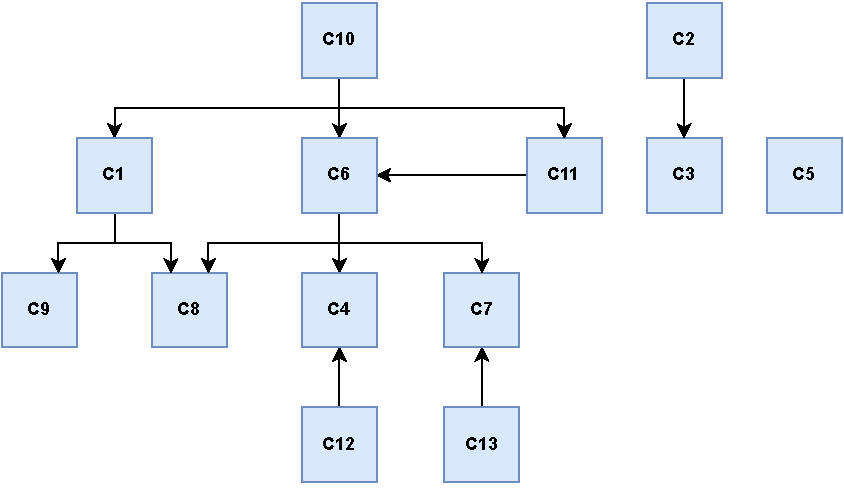
\includegraphics[width=0.87\linewidth]{figures/concept2concept.pdf}
    \caption[Dependencies between Conceptual Models]{Dependencies between
        Conceptual Models (Section~\ref{sec_conceptual})}
    \label{fig:conceptualdependencies}
\end{figure}
\vspace*{\fill}

\vspace*{\fill}
\begin{figure}[tbh]
    \centering
    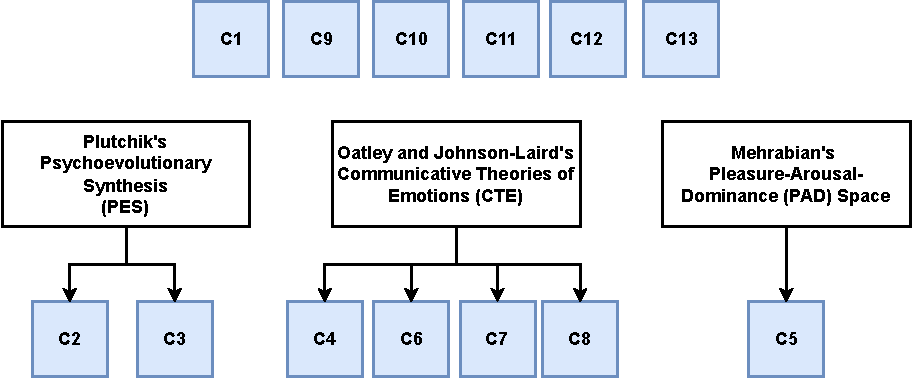
\includegraphics[width=\linewidth]{figures/theories2concept.pdf}
    \caption[Conceptual Model Dependencies on Affective
    Theories/Models]{Conceptual Model Dependencies on Affective Theories/Models
    (Section~\ref{sec_conceptual})}
    \label{fig:theories2conceptual}
\end{figure}
\vspace*{\fill}

\begin{figure}[tbh]
    \centering
    \includegraphics[height=0.96\textheight]{figures/assumptions2All.pdf}
    \caption[Dependencies on Assumptions]{Dependencies on Assumptions (Orange)
    (Section~\ref{sec_assumptions})}
    \label{fig:A2All}
\end{figure}

\begin{landscape}
    \begin{figure}[tbh]
        \centering
        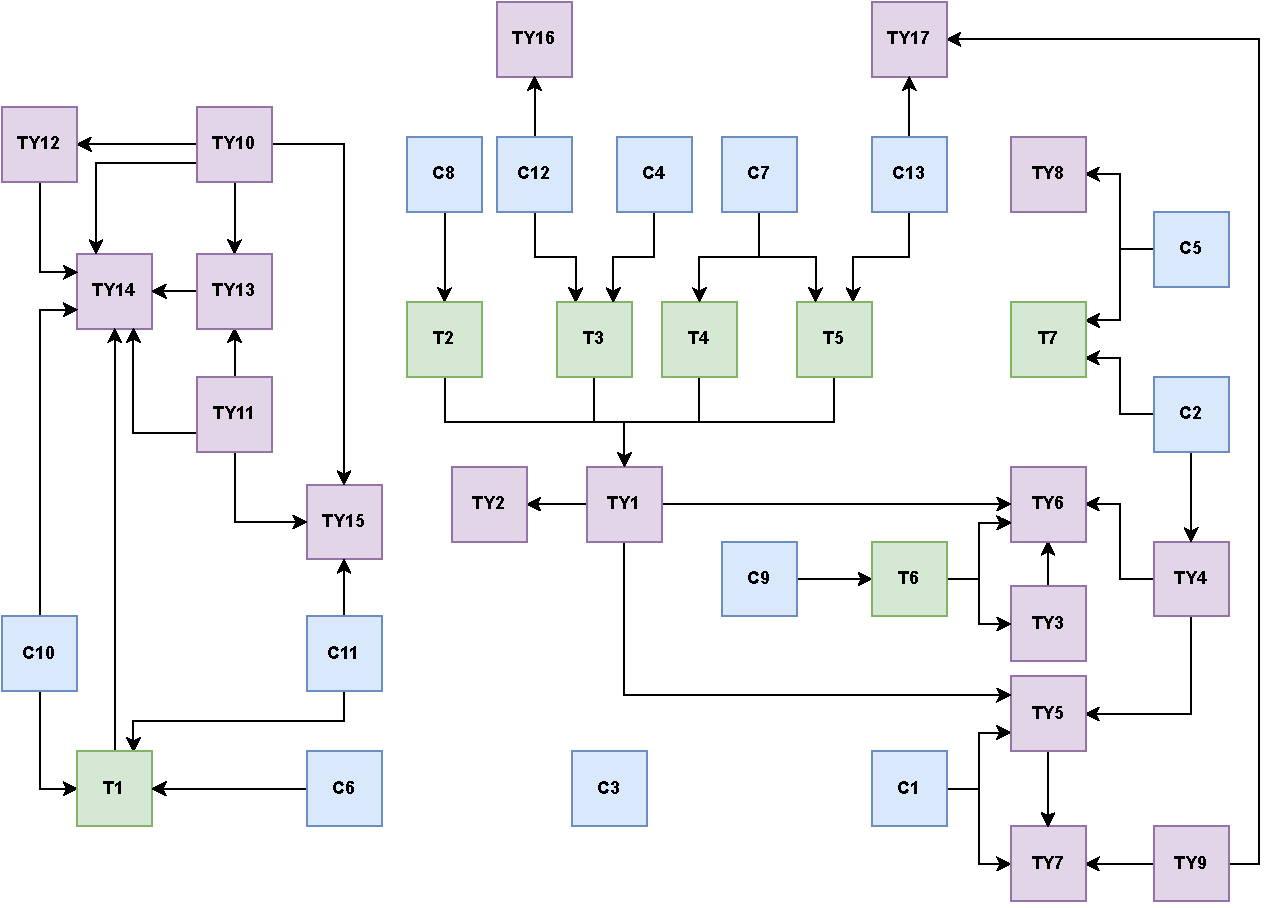
\includegraphics[width=\linewidth]{figures/concept2types_revised.pdf}
        \caption[Traceability between Theoretical Models and Data Types, and
        their dependencies on Conceptual Models]{Traceability between
        Theoretical Models (Green) and Data Types (Purple), and their
        dependencies on Conceptual Models (Blue)
        (Sections~\ref{sec_theoretical}, \ref{sec_typedefs},
        and~\ref{sec_conceptual})}
        \label{fig:C2TY}
    \end{figure}
\end{landscape}

\begin{landscape}
    \begin{figure}[tbh]
        \centering
        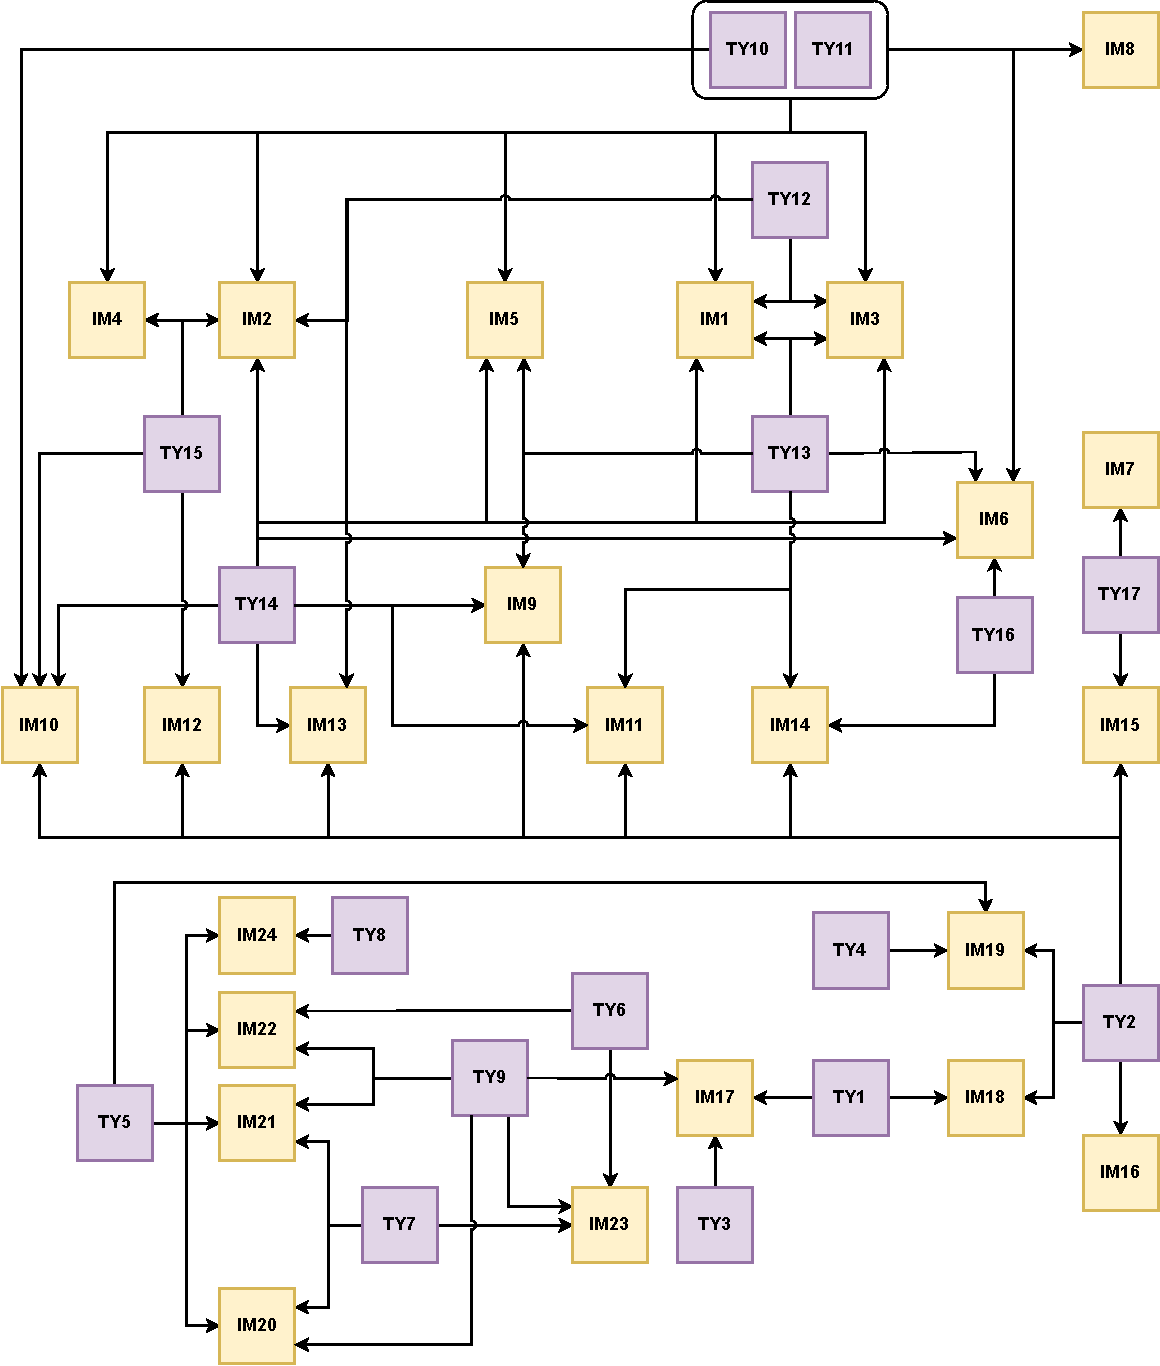
\includegraphics[width=0.88\linewidth]{figures/types2instance.pdf}
        \caption[Instance Models and their Dependencies on Theoretical Models
        and Data Types]{Instance Models (Yellow) and their Dependencies on
        Theoretical Models (Green) and Data Types (Purple)
        (Sections~\ref{sec_theoretical}, \ref{sec_typedefs},
        and~\ref{sec_instance})}
        \label{fig:T-TY2IM}
    \end{figure}
\end{landscape}

\vspace*{\fill}
\begin{figure}[tbh]
    \centering
    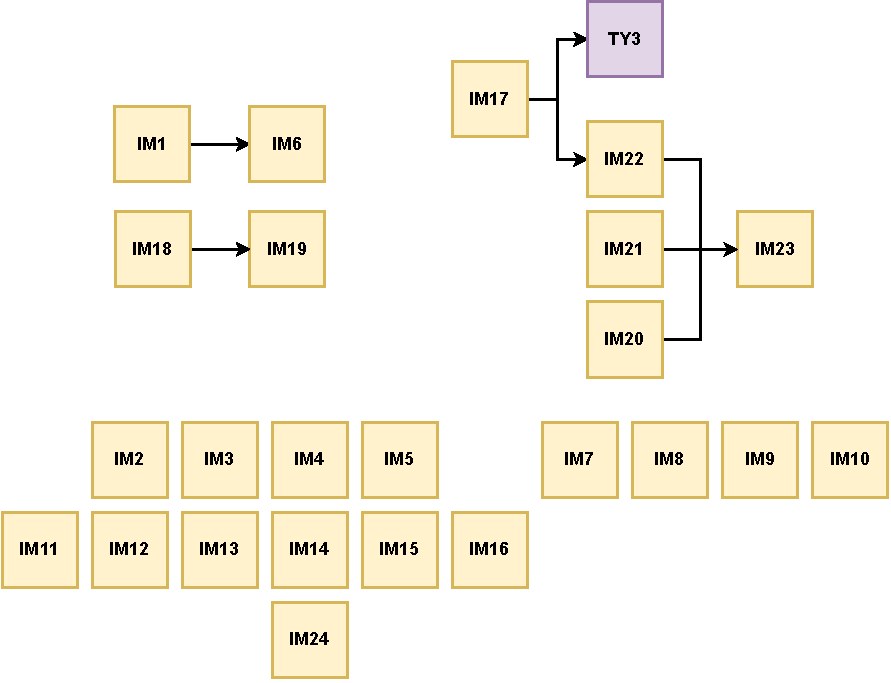
\includegraphics[width=0.5\linewidth]{figures/instance2instance.pdf}
    \caption[Dependencies between Instance Models]{Dependencies between
        Instance Models (Section~\ref{sec_instance})}
    \label{fig:IM}
\end{figure}
\vspace*{\fill}

\begin{figure}[tbh]
    \centering
    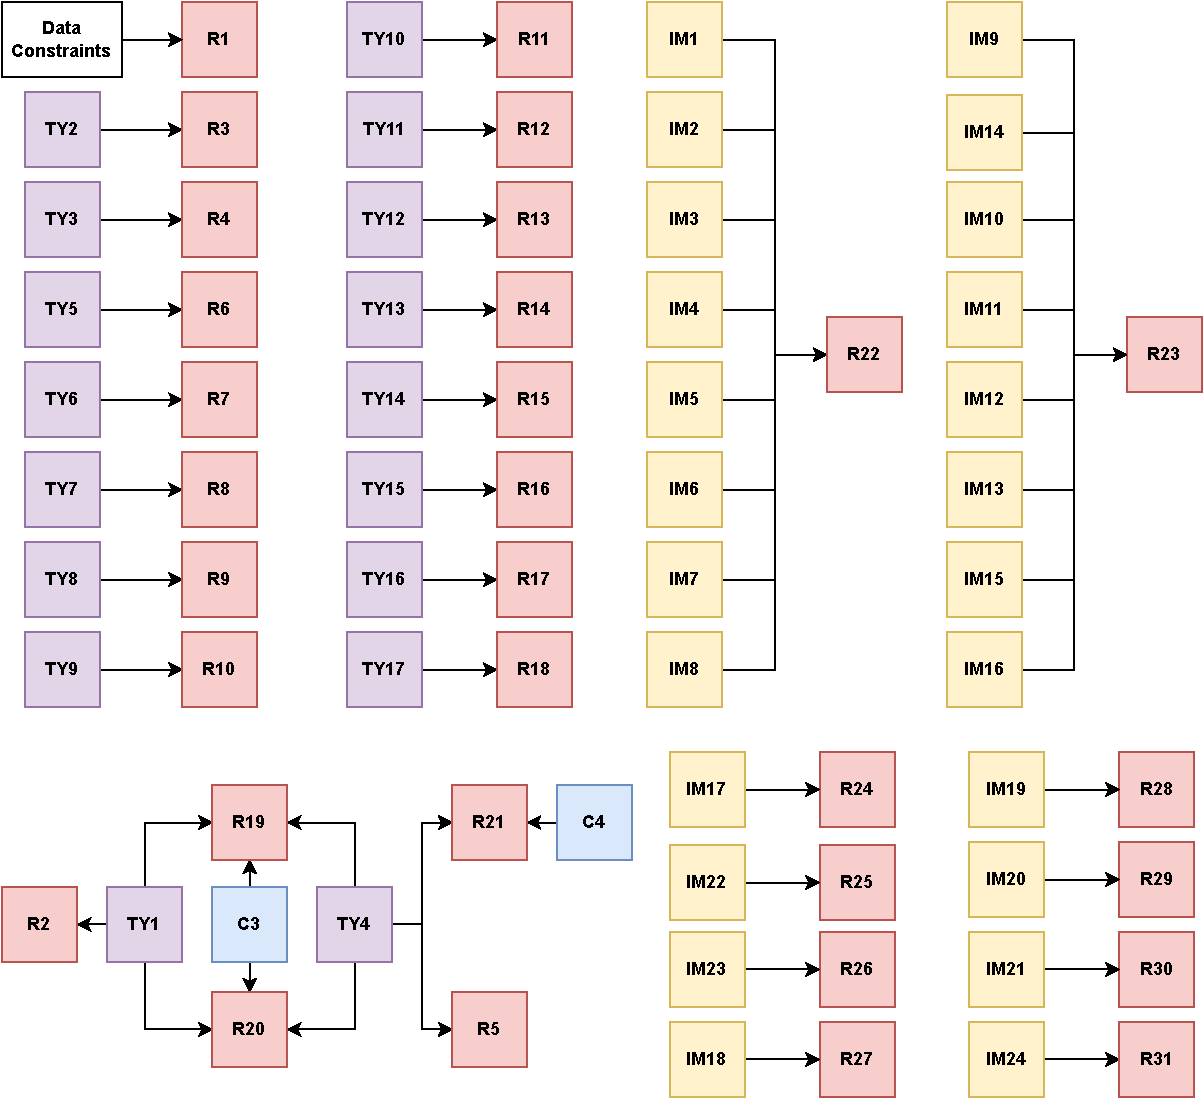
\includegraphics[width=\linewidth]{figures/reqs2All.pdf}
    \caption[Functional Requirements and their Dependencies on Conceptual
    Models, Data Types, Instance Models, and Data Constraints]{Functional
    Requirements (Red) and
    their Dependencies on Conceptual Models (Blue), Data Types (Purple),
    Instance Models (Yellow), and Data Constraints
    (Sections~\ref{sec_conceptual}, \ref{sec_typedefs}, \ref{sec_instance},
    \ref{sec_DataConstraints}, and \ref{sec_functionalreqs})}
    \label{fig:M2R}
\end{figure}